%%%%%%%%%%%%%%%%%%%%%%%%%%%%%%%%%%%%%%%%%
% Beamer Presentation
% LaTeX Template
% Version 1.0 (10/11/12)
%
% This template has been downloaded from:
% http://www.LaTeXTemplates.com
%
% License:
% CC BY-NC-SA 3.0 (http://creativecommons.org/licenses/by-nc-sa/3.0/)
%
%%%%%%%%%%%%%%%%%%%%%%%%%%%%%%%%%%%%%%%%%

%----------------------------------------------------------------------------------------
%	PACKAGES AND THEMES
%----------------------------------------------------------------------------------------

\documentclass{beamer}

\mode<presentation> {

% The Beamer class comes with a number of default slide themes
% which change the colors and layouts of slides. Below this is a list
% of all the themes, uncomment each in turn to see what they look like.

%\usetheme{default}
%\usetheme{AnnArbor}
%\usetheme{Antibes}
%\usetheme{Bergen}
%\usetheme{Berkeley}
%\usetheme{Berlin}
%\usetheme{Boadilla}
%\usetheme{CambridgeUS}
%\usetheme{Copenhagen}
%\usetheme{Darmstadt}
%\usetheme{Dresden}
%\usetheme{Frankfurt}
%\usetheme{Goettingen}
%\usetheme{Hannover}
%\usetheme{Ilmenau}
%\usetheme{JuanLesPins}
%\usetheme{Luebeck}
\usetheme{Madrid}
%\usetheme{Malmoe}
%\usetheme{Marburg}
%\usetheme{Montpellier}
%\usetheme{PaloAlto}
%\usetheme{Pittsburgh}
%\usetheme{Rochester}
%\usetheme{Singapore}
%\usetheme{Szeged}
%\usetheme{Warsaw}

% As well as themes, the Beamer class has a number of color themes
% for any slide theme. Uncomment each of these in turn to see how it
% changes the colors of your current slide theme.

%\usecolortheme{albatross}
%\usecolortheme{beaver}
%\usecolortheme{beetle}
%\usecolortheme{crane}
%\usecolortheme{dolphin}
%\usecolortheme{dove}
%\usecolortheme{fly}
%\usecolortheme{lily}
%\usecolortheme{orchid}
%\usecolortheme{rose}
%\usecolortheme{seagull}
%\usecolortheme{seahorse}
%\usecolortheme{whale}
%\usecolortheme{wolverine}

%\setbeamertemplate{footline} % To remove the footer line in all slides uncomment this line
%\setbeamertemplate{footline}[page number] % To replace the footer line in all slides with a simple slide count uncomment this line

%\setbeamertemplate{navigation symbols}{} % To remove the navigation symbols from the bottom of all slides uncomment this line
}

\usepackage{graphicx} % Allows including images
\usepackage{booktabs} % Allows the use of \toprule, \midrule and \bottomrule in tables
\graphicspath{ {../img/} }%setta il path predefinito per le immagini
\usepackage[utf8]{inputenc}
\usepackage{hyperref}

%----------------------------------------------------------------------------------------
%	TITLE PAGE
%----------------------------------------------------------------------------------------

\title[Trajectory Clustering survey]{Trajectory Clustering Alghorithms - Two scalable and Comovement-based approaches. } % The short title appears at the bottom of every slide, the full title is only on the title page

\author{Federico Naldini} % Your name
\institute[Università di Bologna] % Your institution as it will appear on the bottom of every slide, may be shorthand to save space
{
Alma Mater Studiorum - Università di Bologna, Cesena. \\ % Your institution for the title page
\medskip
\textit{federico.naldini3@studio.unibo.it} % Your email address
}
\date{15/10/2019} % Date, can be changed to a custom date

\begin{document}

\begin{frame}
\titlepage % Print the title page as the first slide
\end{frame}

%------------------------------------------------
\begin{frame}
\frametitle{Overview} % Table of contents slide, comment this block out to remove it
\tableofcontents % Throughout your presentation, if you choose to use \section{} and \subsection{} commands, these will automatically be printed on this slide as an overview of your presentation
\end{frame}
%------------------------------------------------
%----------------------------------------------------------------------------------------
%	PRESENTATION SLIDES
%----------------------------------------------------------------------------------------

%------------------------------------------------
\section{Comovement patterns} % Sections can be created in order to organize your presentation into discrete blocks, all sections and subsections are automatically printed in the table of contents as an overview of the talk

\begin{frame}

\frametitle{Che cosa sono i \textit{Comovements patterns}?}
I \textit{Comovements patterns} sono raggruppamenti di oggetti che hanno viaggiato assieme per un certo periodo di tempo.

L'interesse per questi insieme può essere basato su diversi fattori, come ad esempio il numero degli elementi, la durata del viaggio,
la loro effettiva vicinanza e il criterio utilizzato per calcolarla.

A seconda delle differenti caratteristiche utilizzate nel definire i raggruppamenti, è possibile definire delle tipologie di raggruppamenti.

\end{frame}
%------------------------------------------------

\begin{frame}

\frametitle{Tipologie di \textit{Co-movements pattern}}

Le tipologie di \textit{Co-movements pattern} possono essere divise sulla base di diversi fattori; 
tra tutti spicca in particolare la metrica di similarità utilizzata. 
Possono essere impiegate due misure:

\begin{itemize}

\item \textbf{Similarità basata sulla densità}

\item \textbf{Similarità basata sulla distanza}

\end{itemize}

\end{frame}

\begin{frame}

\frametitle{Similarità basata sulla densità}

\begin{itemize}

\item \textbf{Convoy}: Identifica raggruppamenti di oggetti che hanno percorso traiettorie simili per almeno \textit{T} istanti consecutivi, negli algoritmi classici prima viene applicato un algoritmo di \textit{clustering} basato sulla densità e successivamente viene effettuato \textit{pruning} sulla base del criterio temporale sopraespresso.

\item \textbf{Swarm}: Rispetto a \textbf{Convoy} scarta il vincolo di sequenzialità degli istanti temporali, basandosi solo sui vincoli spaziali.

\item \textbf{Platoon}:Rimuove il vincolo descritto da \textbf{Convoy}, sostituendolo con un vincolo locale sugli istanti consecutivi
tramite un parametro L che identifica la lunghezza 
minima di ogni sottosequenza di istanti consecutivi.

Inoltre aggiunge un altro parametro K, che identifica la lunghezza minima della sequenza temporale \textit{T} di ogni raggruppamento.

  

\end{itemize}

\end{frame}


\begin{frame}

\frametitle{Similarità basata sulla distanza}

\begin{itemize}

\item \textbf{Flock}: La stessa idea presentata in \textbf{Convoy}, ma utilizzando una metrica di similarità basata sulla definizione
di uno spazio chiamato \textit{disk} di raggio \textit{r}.


\item \textbf{Group}:Rilassa il vincolo temporale introdotto da \textbf{Flock} introducendo un vincolo sulla lunghezza delle sequenze di istanti consecutivi, analogamente a quanto fatto in \textit{Platoon}; tuttavia a differenza di quest'ultimo non introduce un vincolo sulla lunghezza totale della sequenza.


\end{itemize}

\end{frame}



%------------------------------------------------

\section{GCMP: un framework generico per il mining di Comovements}

\subsection{Obiettivi e definizione del problema e dei parametri}

\begin{frame}
\frametitle{General Co-movement Patter Mining}
Il framework \textbf{GCMP} si pone come obiettivo di mettere a disposizione degli utilizzatori una piattaforma configurabile per realizzare tutte le tipologie di \textit{Co-movement mining} sopradescritte.

In particolare definisce diversi parametri per la definizione del problema:
\end{frame}

\begin{frame}
\frametitle{General Co-movement Patter Mining: Parametri 1}

\begin{itemize}

\item \textbf{M}: Numero minimo di elementi presenti in un raggruppamento per considerarlo interessante.
\item \textbf{K}: Numero minimo di istanti temporali in cui un certo raggruppamento esiste.

\end{itemize}

\end{frame}

\begin{frame}
\frametitle{General Co-movement Patter Mining: Parametri 2}

\begin{itemize}

\item \textbf{L}: Data una sequenza temporale di istanti \textit{T}, si identificano \textit{z} sottosequenze tali che ogni sottosequenza è composta da istanti consecutivi(ad esempio con \textit{T} = (1,2,3,5,6) si ottengono due sottosequenze \textit{T'} = 
(1,2,3) e \textit{T''} = (5,6)); \textbf{L} identifica la lunghezza minima accettabile di tutte le \textit{z} sottosequenze così individuate(ad esempio con \textbf{L} = 3 la sequenza non rispetta il vincolo, mentre con \textbf{L} = 2 sì).

Una sequenza che rispetta il vincolo sopradescritto viene definita \textit{L-consecutive}
\item \textbf{G}:  Data una sequenza temporale di istanti \textit{T}, \textbf{G} identifica il massimo \textit{skew} accettabile tra un elemento della sequenza e il successivo. Una sequenza si definisce \textit{G-connected} se per ogni coppia di elementi consecutivi al suo interno 
lo \textit{skew} in questione è minore o uguale a \textbf{G} 

\end{itemize}

\end{frame}

\begin{frame}
\frametitle{General Co-movement Patter Mining: Definizione}

Un \textbf{GCPM} trova un set di oggetti \textit{O}, rimasti assieme per una sequenza di istanti \textit{T} che soddisfa i seguenti vincoli:

\begin{itemize}

\item \textit{Closeness}: per ogni istante di \textit{T}, gli oggetti \textit{O} devono appartenere allo stesso \textit{cluster}.
\item \textit{Significance}: La dimensione del raggruppamento deve essere maggiore di \textbf{M}.
\item \textit{Duration}: La dimensione di \textit{T} deve essere maggiore di \textbf{K}.
\item \textit{Consecutiveness}: \textit{T} è \textit{L-consecutive}.
\item \textit{Connection}: \textit{T} è \textit{G-connected}.


\end{itemize}

\end{frame}

\begin{frame}
\frametitle{General Co-movement Patter Mining: Parametri 3}

Configurando i vari parametri, posso ottenere le cinque tipologie di \textit{Co-movements}

\begin{center}
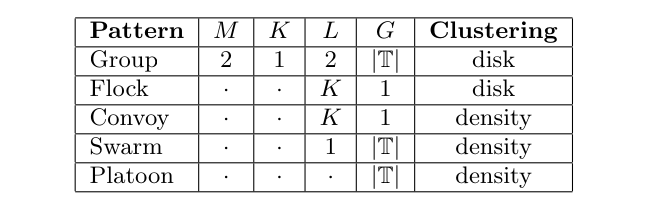
\includegraphics[scale=0.4]{ParametersConfiguration} 
\end{center}

\end{frame}



\subsection{Algoritmo di risoluzione}

\subsubsection{Generazione degli Snapshot}

\subsubsection{Star Partitioning}

\subsubsection{Apriori Enumeration}

\section{Scalable Distribuited Subtrajectory Clustering}




\begin{frame}
\titlepage % Print the title page as the last slide
\end{frame}

%----------------------------------------------------------------------------------------

\end{document}
